\documentclass[a4paper, amsfonts, amssymb, amsmath, reprint, showkeys, nofootinbib, twoside]{revtex4-1}
\usepackage[english]{babel}
\usepackage[utf8]{inputenc}
\usepackage[colorinlistoftodos, color=green!40, prependcaption]{todonotes}
\usepackage[pdftex, pdftitle={Article}, pdfauthor={Author}]{hyperref}
\usepackage{amsthm}
\usepackage{mathtools}
\usepackage{physics}
\usepackage{xcolor}
\usepackage{caption}
\usepackage{hyperref}
%\hypersetup{colorlinks=true, linkcolor=blue, urlcolor = blue}
\usepackage{amsmath}
\usepackage{amssymb}
\usepackage{graphicx}
\graphicspath{Images}
\usepackage[left=23mm,right=13mm,top=35mm,columnsep=15pt]{geometry} 
\usepackage{adjustbox}
\usepackage{placeins}
\usepackage[T1]{fontenc}
\usepackage{float}
%\usepackage{longtable}
\usepackage{csquotes}
\usepackage{refstyle}
\usepackage{lipsum}

\begin{document}

\title{Study of C-V Characteristics of Solar Cell}
\author{Swaroop Ramakant Avarsekar}
\email{swaroop.avarsekar@niser.ac.in}
\affiliation{School of Physical Sciences, National Institute of Science Education and Research, HBNI, Jatni -752050, India}
\date{\today}

	
\begin{abstract}
This experiment aims to study the C-V characteristics of solar cell by reverse biasing and determining the doping density and built in potential of the solar cell. With the p-n junction reverse biased, the solar cell acts as a capacitor. The capacitance profile of solar cell with input voltage is studied. The plot of $V$ versus $1/C^{2}$ is linear. Therefore, the doping density of solar cell under dark and light conditions are $(6.014\pm0.227)\times10^{16}$ SI units and $(8.538\pm0.519)\times10^{16}$ SI units, respectively with built in voltage as $(0.232\pm0.028)$ V and $(0.209\pm0.037)$ V for the former and latter case, respectively.
\end{abstract}
	
\keywords{Built in potential, Doping density, Op-Amp}
	
\maketitle

\section{Theory}
As we know, solar cell is a p-n junction. When it is forward biased V-I characteristics is studied as there is a output voltage due to photovoltaic effect. To enhance the output power, optimal amount of doping is required. To calculate the doping density and built in potential of a solar cell, we study its C-V profile. 

Reverse biasing the p-n junction results in formation of space charge region due to acceptors in the p side and donors on the n side. Due to absence of mobile carriers in this region, free charge carriers respond to external ac voltage applied thus forming a parallel plate capacitor with 
capacitance,

\begin{equation}\label{e1}
	C=\frac{\epsilon A}{x}=\frac{dQ}{dV_{DC}}
\end{equation}

Where $V_{DC}$ is reverse bias voltage, $Q$ si the charge, $A$ is Area of the parallel plate, $\epsilon=\epsilon_o\epsilon_r$ $\epsilon_o$ are $\epsilon_r$ permittivity in free space and medium respectively, x is the width of depletion region.

The width of depletion layer is also given by 

\begin{equation}\label{e2}
	x=\left(\frac{2.\epsilon_o.\epsilon_r.(V_{bi}+V_{DC})}{q.N}\right) ^{1/2}
\end{equation}

where N is the doping density of the solar cell, $V_{bi}$ is the built in potential. 

From equations (\ref{e1}) and (\ref{e2}), we get:

\begin{equation}\label{e3}
	\frac{1}{C^2}=\left(\frac{x}{\epsilon_o.\epsilon_r.A}\right)^{2} =\left(\frac{2.(V_{bi}+V_{DC})}{q.NA^2.\epsilon_o.\epsilon_r}\right) 
\end{equation}

From slope and intercept of linear fit of equation (\ref{e3}), $N$ and $V_{bi}$ can be calculated.

\begin{figure}[H]
	\centering
	\includegraphics[scale=0.3]{1} 
	\caption{Circuit diagram for the C-V characteristics of solar cell. Here, A is anode and K is Cathode of solar cell.}
	\label{1}
\end{figure}

It is evident from the formula that the C of solar cell depends on applied reverse bias voltage. A variable DC voltage along with small AC current is supplied to read the capacitance. Here device under test (DUT) is solar cell. It should be noted that that the AC current should be very small else it may perturb the DC biasing affecting the polarization. This can be done using unity gain amplifier for reverse bias voltage and attenuating the AC signal by 1/10 th by choosing appropriate resistor as shown in figure (\ref{1}) , i.e 10 k$\Omega$. The output voltage for DUT is then given by equation (\ref{dut}),

\begin{equation}\label{dut}
	V_{DUT}=\frac{-R}{R_2}V_{DC}+\frac{-R}{R_1}V_{AC}
\end{equation}

This $V_{DUT}$ is fed to anode of solar cell and cathode is connected to inverting pin of Op-Amp, with the capacitor and resistor as feedback. The current thorugh the capacitor is directly proportinal to the AC signal applied. Use of trans impedance amplifier is necessary as current through capacitor is converted to voltage which can be read in multi-meter, generating a output proportional to solar cell's capacitance ($C_{DUT}$) , which is given by :

\begin{equation}\label{ev}
	V_{out}=\frac{V_{DUT}.C_{DUT}}{C_{f}.\sqrt{1+\frac{1}{(\omega R_f C_f)^2}}}
\end{equation}

Equation (\ref{ev}) can be rearranged to give $C_{DUT}$ as :

\begin{equation}
	C_{DUT}=\frac{V_{out}.C_f.\sqrt{1+\frac{1}{(\omega R_f C_f)^2}}}{V_{DUT}}
\end{equation}

It should be noted that high frequencies must be used as for low frequencies Op-Amp exhibit 1/f noise. Either of Op-Amp IC 741 or TL 071 or TL 072 can be used but the latter is preferred due to low noise, high slew rate. Also, the reverse bias voltage should be varied slowly in steps and experiment should be performed by covering the solar cell with dark cloth. Also, trying with room light help you compare the characteristics.

\section{Experiment}
Experimental setup is shown in Figure (\ref{s}). The C-V characteristics is shown in Figure (\ref{2}). It is seen that the two curves converge at high voltage, but the initial capacitance varies with the light input. The plot of V versus $1/C^{2}$ for solar cell under dark and tube light is shown in figure (\ref{3}) and  (\ref{4}), respectively. 

\begin{figure}[H]
	\centering
	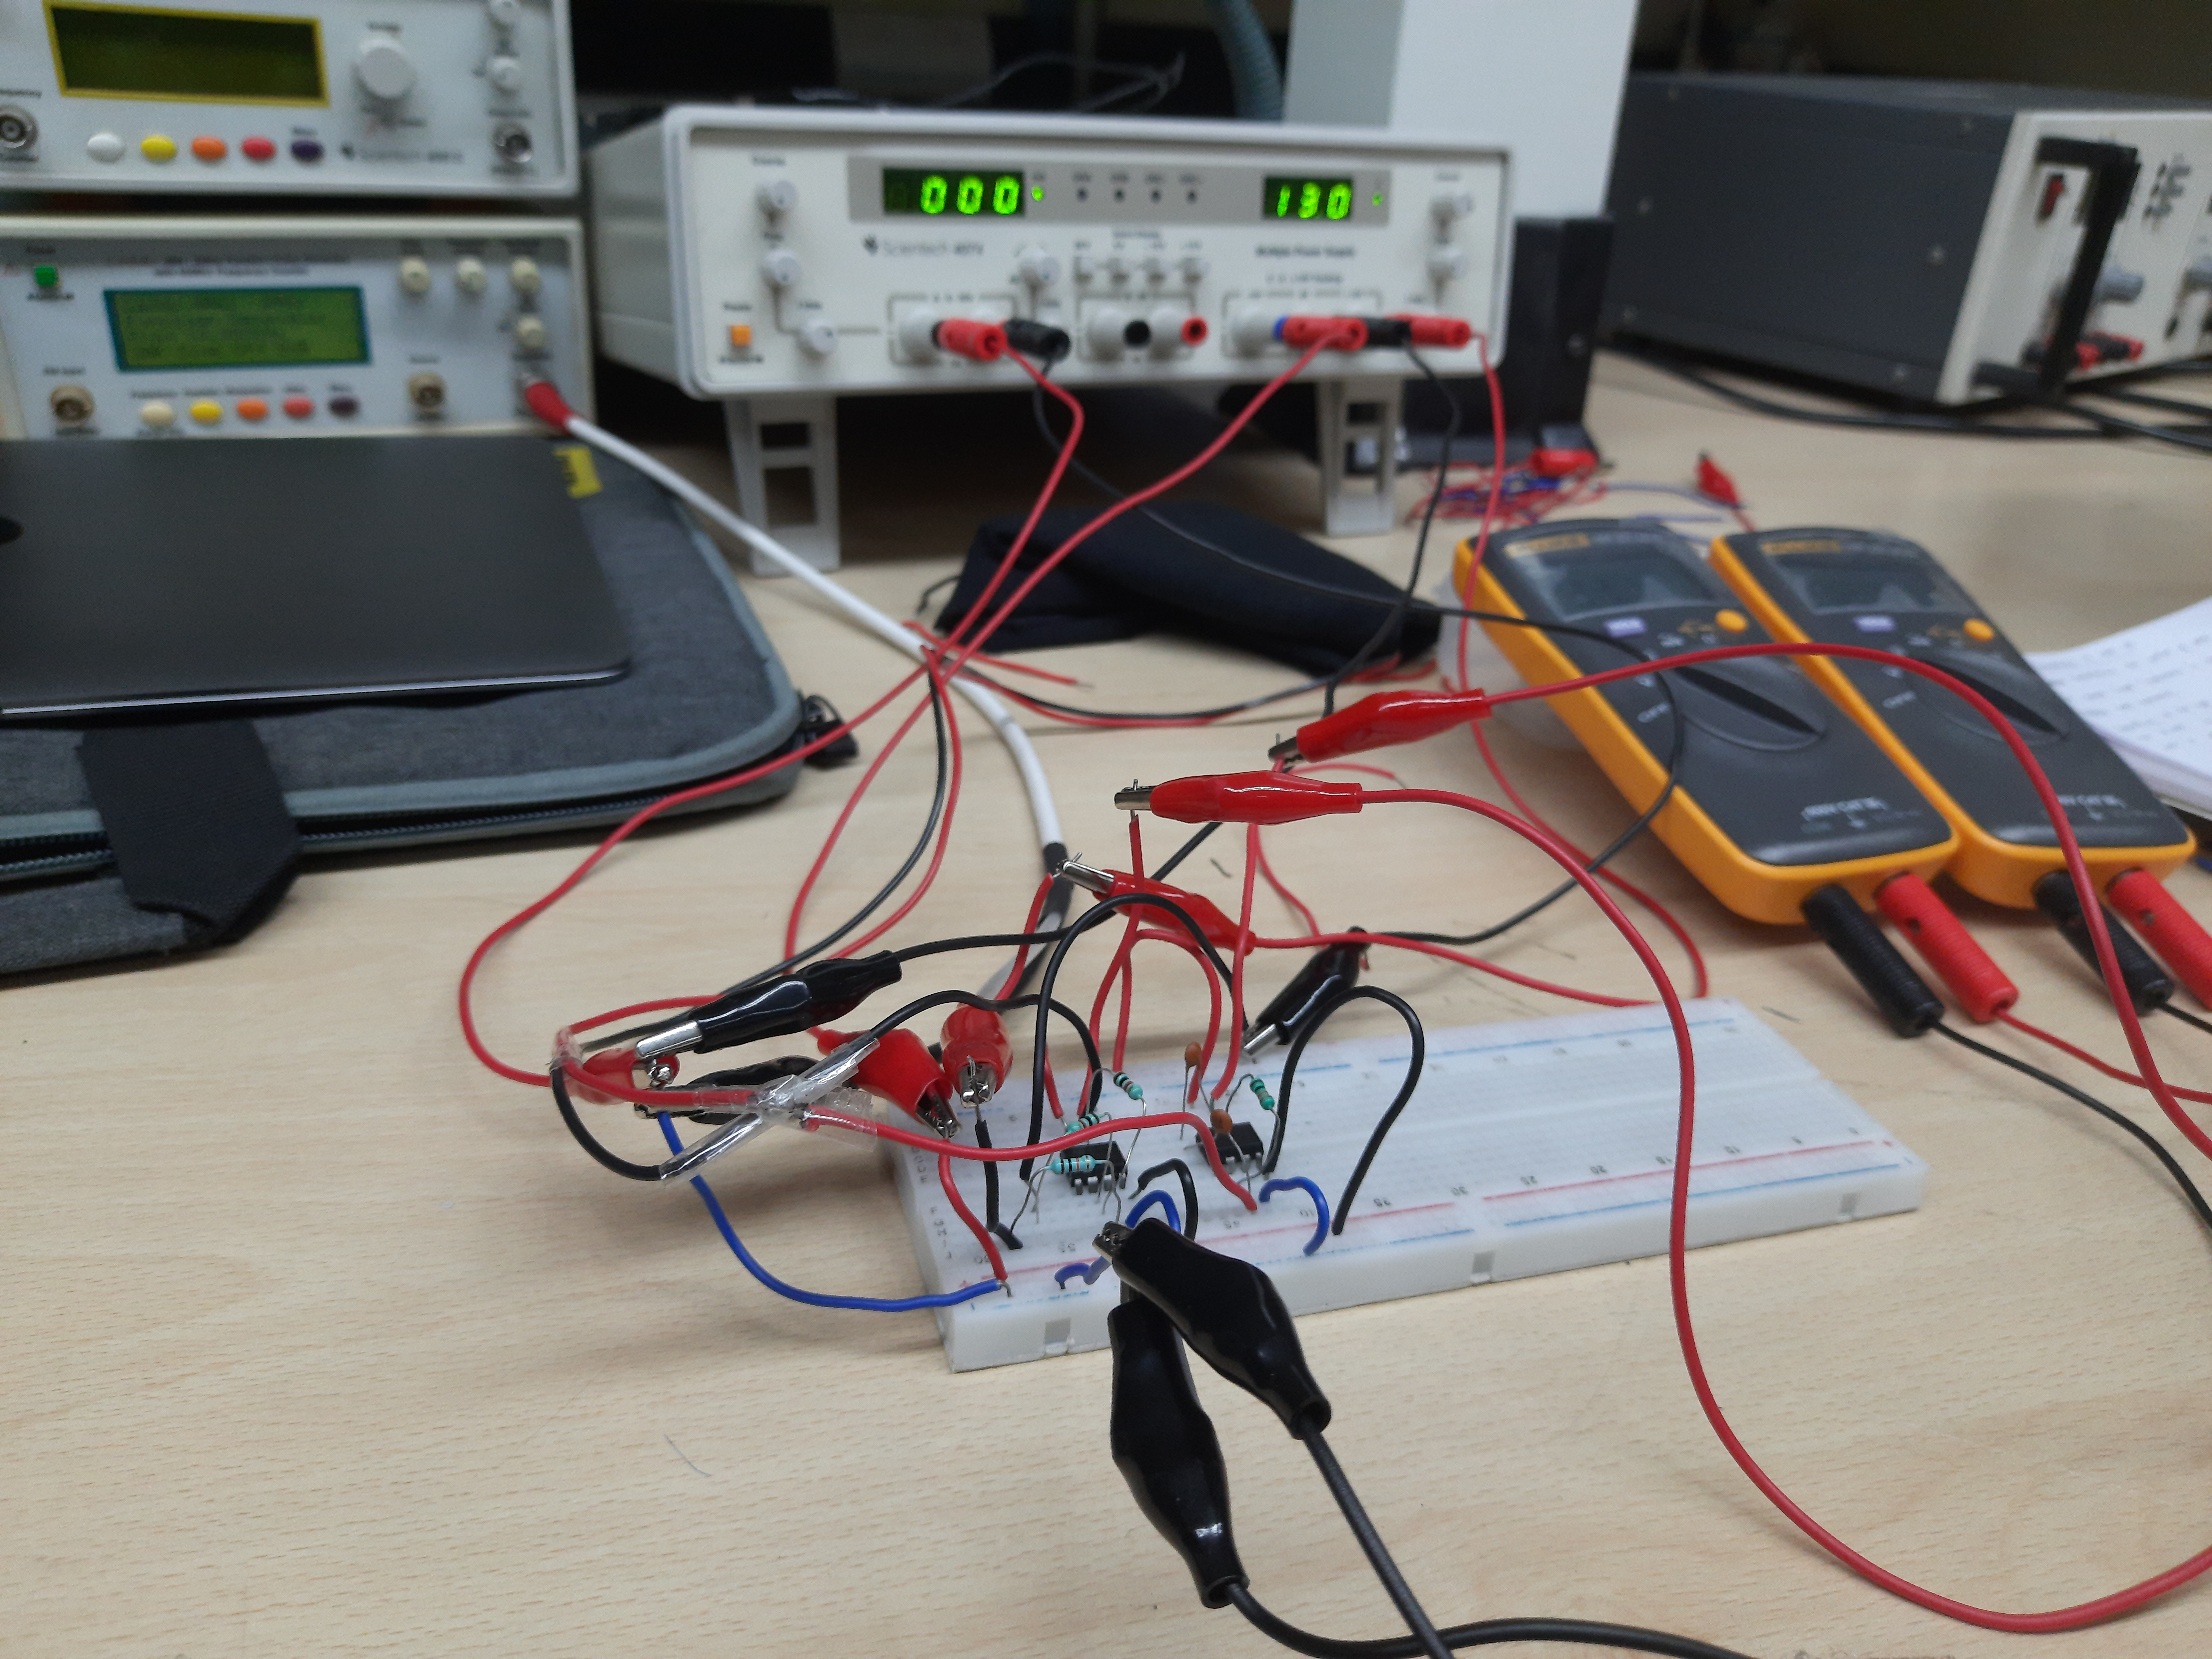
\includegraphics[width=\columnwidth]{setup}
	\caption{Experimental setup at laboratory}
	\label{s}
\end{figure}

\begin{figure}[H]
	\centering
	\includegraphics[scale=0.57]{cv}
	\caption{C-V characteristics of solar cell in different light conditions: Dark and Tube light}
	\label{2}
\end{figure}

\begin{figure}[H]
	\centering
	\includegraphics[scale=0.57]{c2vd}
	\caption{Plot of V versus $1/C^{2}$ for solar cell placed in dark region.}
	\label{3}
\end{figure}

\begin{figure}[H]
	\centering
	\includegraphics[scale=0.57]{c2vtb}
	\caption{Plot of V versus $1/C^{2}$ for solar cell placed in tube light.}
	\label{4}
\end{figure}

\section{Calculation and Analysis}
From the plots as shown in Figure (\ref{3}) and Figure (\ref{4}), the built in potential $ V_{bi} $ and doping density $ N $ can be calculated from the slope and intercept.

From equation (\ref{e3}) doping density and built in potential equates as given in equation (\ref{n}) and (\ref{vb}):

\begin{equation}\label{n}
	N=\frac{2}{e.A^{2} \epsilon_o\epsilon_r.m}
\end{equation}

where e is charge of electron and m is slope.

\begin{equation}\label{vb}
	V_{bi}=\frac{e.N.A^{2} \epsilon_o\epsilon_r.c}{2}
\end{equation}
where c is y intercept.

The area of solar cell was measured to be 19.61 $cm^{2}$ and dielectric constant as 11.7. Substituting all the values to get N and $V_{bi}$.

For solar cell under dark,

\begin{equation}
	N_{dark}=\frac{2}{e.(19.61\times10^{-4})^{2} \epsilon_o.(11.7)(0.521\times10^{18})}
\end{equation}

Doping density, $N_{dark}=6.014\times10^{16}$ SI units

Error in $N_{dark}$:
\begin{equation}
	\frac{\delta N_{dark}}{ N_{dark}}=\sqrt{\left( \frac{2.\delta A}{A}\right) ^{2}+\left( \frac{\delta m}{m}\right) ^{2}}
\end{equation}

\begin{equation}
	\frac{\delta N_{dark}}{ 6.014\times10^{16}}=\sqrt{\left( \frac{2\times0.1}{19.61}\right) ^{2}+\left( \frac{0.019}{0.521}\right) ^{2}}
\end{equation}

$\delta N_{dark}$=0.227$\times10^{16}$ SI units

\begin{equation}%\label{vb}
	V_{bi_{dark}}=\frac{e.(6.014\times10^{16}).A^{2} \epsilon_o.(11.7)(0.121\times10^{18})}{2}
\end{equation}

Built in potential, $V_{bi_{dark}}$ is 0.232 V

Error in $V_{bi_{dark}}$:
\begin{equation}
	\frac{\delta V_{bi_{dark}}}{ V_{bi_{dark}}}=\sqrt{\left( \frac{2.\delta A}{A}\right) ^{2}+\left( \frac{\delta N_{dark}}{N_{dark}}\right) ^{2}+\left( \frac{{\delta c}}{c}\right) ^{2}}
\end{equation}

\begin{equation}
	\frac{\delta V_{bi_{dark}}}{ 0.232}=\sqrt{\left( \frac{2\times0.1}{19.61}\right) ^{2}+\left( \frac{0.227}{6.014}\right) ^{2}+\left( \frac{{0.014}}{0.121}\right) ^{2}}
\end{equation}

$\delta V_{bi_{dark}}$=0.028 V
\newline
\\
For solar cell under light,

\begin{equation}
	N_{light}=\frac{2}{e.(19.61\times10^{-4})^{2} \epsilon_o.(11.7)(0.367\times10^{18})}
\end{equation}

Doping density, $N_{light}=8.538\times10^{16}$ SI units

Error in $N_{light}$:
\begin{equation}
	\frac{\delta N_{light}}{ N_{light}}=\sqrt{\left( \frac{2.\delta A}{A}\right) ^{2}+\left( \frac{\delta m}{m}\right) ^{2}}
\end{equation}

\begin{equation}
	\frac{\delta N_{light}}{ 8.538\times10^{16}}=\sqrt{\left( \frac{2\times0.1}{19.61}\right) ^{2}+\left( \frac{0.022}{0.367}\right) ^{2}}
\end{equation}

$\delta N_{light}$=0.519$\times10^{16}$ SI units

\begin{equation}\label{vbl}
	V_{bi_{light}}=\frac{e.(8.538\times10^{16}).A^{2} \epsilon_o.(11.7).(0.077\times10^{18})}{2}
\end{equation}

Built in potential, $V_{bi_{light}}$ is 0.209 V

Error in $V_{bi_{light}}$:
\begin{equation}
	\frac{\delta V_{bi_{light}}}{ V_{bi_{light}}}=\sqrt{\left( \frac{2.\delta A}{A}\right) ^{2}+\left( \frac{\delta N_{light}}{N_{light}}\right) ^{2}+\left( \frac{{\delta c}}{c}\right) ^{2}}
\end{equation}

\begin{equation}
	\frac{\delta V_{bi_{light}}}{ 0.209}=\sqrt{\left( \frac{2\times0.1}{19.61}\right) ^{2}+\left( \frac{0.519}{8.538}\right) ^{2}+\left( \frac{{0.013}}{0.077}\right) ^{2}}
\end{equation}

$\delta V_{bi_{light}}$=0.037 V
\\
\\
Therefore, the doping density of solar cell under dark and light conditions are $(6.014\pm0.227)\times10^{16}$ SI units and $(8.538\pm0.519)\times10^{16}$ SI units, respectively with built in voltage as $(0.232\pm0.028)$ V and $(0.209\pm0.037)$ V for the former and latter case, respectively.

\section{Conclusion}
We studied C-V profile of solar cell and successfully determined the doping density and built in potential of it. The circuit was constructed using Op-Amp 741. The doping density N of solar cell under dark and light conditions are $(6.014\pm0.227)\times10^{16}$ SI units and $(8.538\pm0.519)\times10^{16}$ SI units, respectively with built in voltage was found out to be $(0.232\pm0.028)$ V and $(0.209\pm0.037)$ V for the former and latter case. It is seen that the built in potential is closely corresponds to value of Ge as 0.3 V. However the value could be improved by the use of TL 071 as it has low noise with high slew rate. The error could also be reduced by giving the stable sinusoidal frequency from the function generator. 

\section{References}
\begin{enumerate}
\item{\url{https://www.niser.ac.in/sps/sites/default/files/basic_page/p347_2023/8.CV_characeristics_Solarcell.pdf}}
\item {\url{https://aapt.scitation.org/doi/pdf/10.1119/1.5052360}}
%\item {\url{}}


\end{enumerate}

\end{document}